\documentclass{beamer}
\usetheme{metropolis}
\usepackage{amssymb}
\usepackage{graphicx}	
\usepackage{float}
\usepackage{physics}
\usepackage{multirow}
\usepackage{amsfonts,amsmath,oldgerm,algorithmic,algorithm}
\usepackage{appendixnumberbeamer}
\usepackage[font=small,labelfont=bf]{caption} % Required for specifying captions to tables and figures

%\newcommand{\hrefcol}[2]{\textcolor{uihteal}{\href{#1}{#2}}}
\newcommand{\testcolor}[1]{\colorbox{#1}{\textcolor{#1}{test}}~\texttt{#1}}

% Please see Section 18.1 of Beamer User Guide for all the options \usefonttheme provides
\usefonttheme[onlymath]{serif}
% \usefonttheme{serif} % use this if you would like Serif font throughout (and not just for math)

\title{Local magnetic field in a Kondo model leads to impurity phase transition}
%\titlebackground{images/uic_halls.jpg}
% an asterisk will split the background:
% \titlebackground*{images/uic_seo.jpg}
\subtitle{RPC Presentation 2022-23}

\author{{Debraj Debata \\[1mm]{\small Supervisor : Dr. Siddhartha Lal}}}
\date{July 14, 2023}


\usepackage{tikz}
\usetikzlibrary{positioning}
\titlegraphic{
\begin{tikzpicture}[overlay,remember picture]
\node[below right= 2.7 cm] at (current page){
    \includegraphics[width=2cm]{EPQM.pdf}
    \hspace{0cm}
    \includegraphics[width=2cm]{IISER-K_logo.png}
};
\end{tikzpicture}
}



\begin{document}

\maketitle


% default is no footline, but page numbers are incredibly useful for the audience to ask questions later
%\footlinecolor{uicblue}


\begin{frame}{Motivation for the project}
\begin{figure}[!ht]
    \centering
    \includegraphics[scale=1.2]{3-orbital-DMFT.pdf}
    \caption{DMFT}
\end{figure}
\end{frame}


\begin{frame}{Motivation for the project}
\begin{figure}[!ht]
    \centering
    \includegraphics[scale=0.6]{3-orbital-model-1.pdf}
    \includegraphics[scale=0.6]{3-orbital-model-2.pdf}
    \includegraphics[scale=0.6]{3-orbital-model-3.pdf}
    \includegraphics[scale=0.6]{3-orbital-model-4.pdf}
\end{figure}
\end{frame}

\begin{frame}{Motivation for the project}
\begin{figure}[!ht]
    \centering
    \includegraphics[scale=0.6]{3-orbital-final-model.pdf}
\end{figure}
\end{frame}


\begin{frame}{Application of URG on Impurity Model}
\begin{itemize}
\item It's interesting to understand the physics of Kondo Effect in the presence of magnetic field using non-perturbative Unitary Renormalisation Group(URG) 
\item This previously done by Costi. We reinvestigate the problem and try to not only reproduce old results but also produce some new results with the help of URG.
\end{itemize}
\begin{figure}[!ht]
    \centering
    \includegraphics[scale=0.17]{S2.png}
    \caption{{\small Splitting of the Kondo resonance with increasing magnetic field at $T=0$ and $T/T_K = 0.36$, {\small \textcolor{mLightGreen}{T. A. Costi, PRL, 85, 1504 (2000)}}}}
\end{figure}
\end{frame}

\begin{frame}{Unitary Renormalisation Group(URG)}
\begin{itemize}
\item RG scheme which proceeds by unitary transformations that decouple high-energy k-states
\item Leads to fixed-point Hamiltonians that describe emergent IR physics
\end{itemize}
\begin{figure}[!ht]
    \centering
    \includegraphics[scale=0.35]{URG_transformation.pdf}
    \caption{Scaling concept: Low-energy model Hamiltonians are obtained from the detailed original model by integrating out the high-energy degrees of freedom.}
\end{figure}

\end{frame}


\begin{frame}{Process of Unitary Renormalisation}
\begin{columns}[c]
\begin{column}{.6\textwidth}
\begin{figure}[!ht]
    \centering
    \includegraphics[scale=0.5]{URG_1.pdf}
    \caption{URG process }
\end{figure}
\end{column}
\begin{column}{.6\textwidth}
\begin{figure}[!ht]
    \centering
    \includegraphics[scale=0.5]{URG_2.pdf}
    \caption{URG emergent window and decoupled IOMs}
\end{figure}
 $ \hspace{1cm} U_{(j)}  = \exp \{\frac{\pi}{4}(\eta^\dagger(j) - \eta(j)) \} $ \\
 $\eta^\dagger(j) = \frac{1}{\hat{w}_{(j)} - Tr(H_{(j)} \hat{n}_{j})} c_j^\dagger Tr(H_{(j)}c_j)  $
 \vspace{0.2cm}
 
 {\small \textcolor{mLightGreen}{ \hspace{5mm} A. Mukherjee and S. Lal, Nuclear Physics B 960, 115170 \& 115163 (2020)}}
\end{column}
\end{columns}
\end{frame}



\begin{frame}{Kondo Model in Local Magnetic Field}
\begin{itemize}
\item The Kondo effect is an unusual mechanism of conduction electrons in a metal due to magnetic impurities
\item  It's one of the key concept in understanding the behavior of metallic systems with strongly interacting electrons.
\end{itemize}
\begin{figure}[!ht]
    \centering
    \includegraphics[scale=0.25]{Kondo.pdf}
    \caption{Kondo Effect}
\end{figure}
Kondo Effect in local magnetic field Hamiltonian is described by :\\ $H = \sum_{k,\sigma} \varepsilon_k n_{k \sigma} + J S_d. S_0  + B \mu_B S_d^z$. \\
\end{frame}

\begin{frame}{RG Equations for Kondo in B-field}
RG Equations calculated from URG:
\begin{equation*}
\frac{\Delta J}{\Delta D} =- J^2 \frac{\Tilde{w}}{\Tilde{w}^2 - (\frac{\mu_B B}{2})^2}
\end{equation*}
 \begin{equation*}
 \frac{\Delta B} {\Delta D}=- \frac{J^2}{4} \frac{B}{\Tilde{w}^2 - (\frac{\mu_B B}{2})^2}
 \end{equation*}
$\Tilde{w}^2 = (\frac{\mu_B B}{2})^2$ is the \alert{fixed point} condition where $\Tilde{w} = w - \frac{\varepsilon_q}{2} + \frac{J}{4}$. 
\begin{figure}[!ht]
    \centering
    \includegraphics[scale=0.23]{bitmap2.pdf}
    \caption{Graph when coupling $J$ and $B$ are relevent/irrelevant.}
\end{figure}
\end{frame}

\begin{frame}{Graphical Nature of RG Equations}
Two regions: 
\begin{itemize}
\item \alert{Screened Kondo} region where  $J$ is relevant and $B$ is irrelevant
\item \alert{Local moment} region where $B$ is relevant and $J$ is irrelevant. 
\end{itemize}
\begin{figure}[!ht]
    \centering
    \includegraphics[scale=0.21]{Hari_1_slide.pdf}
    \includegraphics[scale=0.21]{Hari_2_slide.pdf}
    \caption{Initial magnetic field $B_0=2.5$ gives us the idea of \alert{S}creened Kondo behaviour and $B_0 = 20$ for \alert{L}ocal moment behaviour.}
\end{figure}
\end{frame}

\begin{frame}{Impurity Phase Transition   {\hfill\includegraphics[width=4cm]{QF_to_QPT.pdf}\hfill}}

\begin{figure}[!ht]
    \centering
    \includegraphics[scale=0.6]{Quantum-classical transition.pdf}
    \caption{{\small Singlet state becomes polarised state in the presence of B-field}}
\end{figure}

Screened Kondo effective Hamiltonian is :
 $ H = \sum_{ |k|< \Lambda,\sigma} \varepsilon_k n_{k \sigma} + J^* S_d \cdot S_0 $.

Local moment effective Hamiltonian is : 
$ H = \sum_{|k| < \Lambda, \sigma} \varepsilon_k n_{k \sigma} + B^* \mu_B S_d^z$.

\begin{figure}[!ht]
    \centering
    \includegraphics[scale=0.3]{Q-to-C_transition.pdf}
    \caption{{\small Quantum to classical transition due to the presence of magnetic field. Here $g=\frac{\mu_B B}{J}$.}}
\end{figure}

\end{frame}

\begin{frame}{Zero-bandwidth Result}
Zero-bandwidth Hamiltonian : $H = J S_d. S_0 + B \mu_B S_d^z$
\begin{itemize}
\item Zero-momentum model allows singlet and polarised states to becomes degenerate at $g_c \to \infty$ . 
\item Becomes \alert{finite} when dispersion taken into account.
\end{itemize}
\begin{figure}[!ht]
    \centering
    \includegraphics[scale=0.28]{KM_Zero-mode.pdf}
    \caption{Variation of four energies with dimensionless $g=\frac{\mu_B B}{J}$}
\end{figure}
\end{frame}

\begin{frame}{Impurity Magnetization {\hfill\includegraphics[width=4cm]{QF_to_Frustration.pdf}\hfill}}

\metroset{block=fill}
Impurity magnetization : 
 $\langle S_d^z \rangle = - \frac{1}{2}\frac{g^2 +g \sqrt{1+g^2}}{1+ g^2+ g\sqrt{1 + g^2}} $ \
 
 \begin{exampleblock}{For $g=0$ :}
         $\langle S_d^z \rangle$ is $0$, matches with Kondo Effect singlet state.
 \end{exampleblock}
 \begin{exampleblock}{For large $g$ :}
         local moment state, $|\langle S_d^z \rangle| =\frac{1}{2}$
 \end{exampleblock}


\begin{figure}[!ht]
    \centering
    \includegraphics[scale=0.23]{KM_Zero1-mode_slide_S_d_z_1.pdf}
    \caption{{\small $|\langle S_d^z \rangle|$  with variation of $g$}}
\end{figure}



\end{frame}



\begin{frame}{Entanglement Entropy(EE){\hfill\includegraphics[width=4cm]{QF_to_Frustration.pdf}\hfill}}
\begin{columns}[T,onlytextwidth]
 \column{0.5\textwidth}
 \metroset{block=fill}
\begin{exampleblock}{Density Matrix : }
$
\rho_d =\begin{bmatrix}
\frac{1}{2} + \langle S_d^z \rangle & 0 \\
0 & \frac{1}{2} - \langle S_d^z \rangle
\end{bmatrix}
$
\end{exampleblock}
\begin{exampleblock}{Entanglement Entropy}
 (EE)= $ -\rho_d \ln \rho_d$
 \end{exampleblock}
\begin{itemize}
\item Maximally entangled entropy($\ln 2$) for $g = 0$ . 
\item For large $g$, EE is $0$ which gives us information about local moment state. 
\end{itemize}

\column{0.5\textwidth}
\begin{figure}[!ht]
    \centering
    \includegraphics[scale=0.25]{KM_Zero1-mode_slide_EE_1.pdf}
    \caption{{\small EE varies with $g$}}
\end{figure}
\end{columns}
\end{frame}


\begin{frame}{Nature of Gapless Excitation}
Hamiltonian for gapless excitation : $H = J S_d. S_0  + B \mu_B S_d^z -t \sum_\sigma (c_{0\sigma}^\dagger c_{1\sigma} + h.c.) $

\metroset{block=fill}
\begin{alertblock}{\texttt{\textit{At the Critical Point :}}}
 Non-Fermi liquid term, Fermi liquid term and local moment term observed.
\end{alertblock}
Fermi-liquid term at the critical point nicely connected with Fermi-liquid side term. Same for at polarised state side.

\begin{figure}[!ht]
    \centering
    \includegraphics[scale=0.4]{4th_order.pdf}
    \caption{$H_{FL}$: effective Hamiltonian for Fermi-liquid region, $H_{CP}$: for Critical region and local moment region gives $H_{LM}$.}
    \label{olkh}
\end{figure}
\end{frame}



\begin{frame}{Thermalisation at T=0  {\hfill\includegraphics[width=4cm]{QF_to_Decoherence.pdf}\hfill}}
\begin{itemize}
\item This model shows a mechanism for \alert{thermalisation} of pure impurity states into mixed states due to connection to the bath. 
\item An initial separable state $ \ket{\uparrow_d} \otimes \ket{\psi_{rest}}$ ends up in an entangled state:
\begin{align*}
\ket{\uparrow_d \downarrow_0} = \frac{1}{\sqrt{2}} \frac{1}{\sqrt{1+g^2+g\sqrt{1+g^2}}} \Big[(g+\sqrt{1+g^2}) \ket{\Tilde{st}_0} - \ket{\Tilde{ss}} \Big]
\end{align*}
\end{itemize}
\end{frame}

\begin{frame}{Thermalisation at T=0  {\hfill\includegraphics[width=4cm]{QF_to_Decoherence.pdf}\hfill}}
Thermalisation can be seen in the fact that both diagonal entries of \alert{impurity density matrix} acquire non-vanishing values with time. 
\begin{align*}
\begin{pmatrix}
1 & 0\\
0 & 0
\end{pmatrix} \underrightarrow{\text{time dynamics of }\rho_d} \begin{pmatrix}
A(t) & 0\\
0 & D(t)
\end{pmatrix}
\end{align*}
{\small where $A(t) = P_+ + 4 \langle S_d^z \rangle^2  P_-$ and $D(t) =(1 - 4 \langle S_d^z \rangle^2)  P_-$ and $P_{\pm} = \frac{1}{2} \left( 1 \pm \cos wt \right)$.}
\end{frame}


\begin{frame}{Thermalisation at T=0  {\hfill\includegraphics[width=4cm]{QF_to_Decoherence.pdf}\hfill}}
\begin{itemize}
\item {\small The rate of thermalisation $\mathbf{\omega}$ can be controlled by tuning the magnetic field, as shown in Fig below}
\end{itemize}
\begin{figure}[!ht]
    \centering
    \includegraphics[scale=0.18]{KM_time_1_slide.pdf}
    \includegraphics[scale=0.18]{KM_time_2_slide.pdf}
    \includegraphics[scale=0.15]{KM_time_3_slide.pdf}
    \caption{{\small Time evolution of $A$ and $D$ for different $\langle S_d^z \rangle$ : \textbf{Upper left} for $\langle S_d^z \rangle =0 $, \textbf{upper right} for $\langle S_d^z \rangle = 0.25$ and \textbf{below} for $\langle S_d^z \rangle=0.5$.}}
    \label{0okm}
\end{figure}
\end{frame}





\begin{frame}{Present Status \& Future Plan}
\begin{itemize}
\item implementing MERG, a wavefunction based renormalization group where for this project entangled state morphed into polarised state 
\item extending this project by adding bath($0$-th site) magnetic  field
\item In the upcoming months, we will look into potential auxiliary models that can describe a  QCP in the bulk
\end{itemize}
\end{frame}

\begin{frame}{Acknowledgement and Thanks}
\begin{itemize}
\item I would like to thank to my supervisor Dr. Siddhartha Lal for giving me this prototype toy problem which is connected to vast field of physics. Special thanks to him as I also gained various physics knowledge from him beyond my project.
\item I am also greatful to my senior Abhirup da (collaborator of this project also) for a lot of scientific discussions and suggestions.
\end{itemize}

\begin{figure}[!ht]
    \flushright
    \includegraphics[scale=0.18]{THANK_YOU.jpg}
\end{figure}
\end{frame}



% backup slides

\appendix
\begin{frame}
\end{frame}


\begin{frame}{Nature of Gapless Excitation(2nd order)}

\textbf{For 2nd Order}\\
At second order, excitations are described by anisotropic Heisenberg model :
\begin{equation*}
H^{eff} = \mathcal{J}^{\perp} (S_{gs}^- S_1^+ + S_{gs}^+ S_1^-) + \mathcal{J}^z S_{gs}^z S_1^z +    \mathcal{H}_0^1 S_{gs}^z + \mathcal{H}_0^2 S_1^z + C 
\end{equation*}
\begin{itemize}
\item In absence of B-field, impurity (d) and 0 site maximally entangled
\item At critical point, due to degeneracy, entanglement gets shared between impurity, 0 and 1 sites.
\item It tells us that Kondo cloud statrs destroying.
\end{itemize}
\end{frame}

\begin{frame}{Nature of Gapless Excitation(4th Order)}
\textbf{4th order calculation at the critical point}:
{\small \begin{align*}
& \ket{\mathcal{A}} \bra{\mathcal{A}} \Biggl[ Y_3 + (N_1-Y_3)  \ket{\uparrow_1} \bra{\uparrow_1} -Y_3 \ket{\downarrow_1 } \bra{\downarrow_1 }   \Biggl] \\& + \ket{\mathcal{B}} \bra{\mathcal{B}} \Biggl[ Y_5 + (Y_4 -Y_5)  \Big( \ket{0_1} \bra{0_1} + \ket{\uparrow_1 \downarrow_1} \bra{\uparrow_1 \downarrow_1} \Big)  +( N_2 - Y_5 ) \ket{\downarrow_1} \bra{\downarrow_1} \Biggl] \\& + A_0^2 b_1 \Big( Y_1 (\lambda_+ - a_1) + Y_2 (\lambda_- - a_1) \Big) \Big(\ket{\mathcal{A}} \bra{\mathcal{B}} \ket{\uparrow_1} \bra{\downarrow_1}  + \ket{\mathcal{B}} \bra{\mathcal{A}} \ket{\downarrow_1} \bra{\uparrow_1}\Big) 
\end{align*}}
{\footnotesize where, $N_1 = A_0^2 b_1^2 (Y_1 + Y_2)$ and $N_2 = A_0^2 Y_1 (\lambda_+ - a_1)^2 + A_0^2 Y_2 (\lambda_- - a_1)^2$.}\\

\textbf{4th order calculation at Fermi liquid side:}
\begin{align*}
\ket{\mathcal{B}} \bra{\mathcal{B}} \Big[ Y_5 + (Y_4 - Y_5) (\ket{0_1} \bra{0_1} + \ket{\uparrow_1 \downarrow_1} \bra{\uparrow_1 \downarrow_1} ) + (Y_6 - Y_5) \ket{\downarrow_1} \bra{\downarrow_1} \Big] 
\end{align*}
\textbf{4th order calculation at local moment side :}
\begin{align*}
\ket{\mathcal{A}}\bra{\mathcal{A}} \Big(Y_3 + W_1 \ket{\uparrow_1} \bra{\uparrow_1} -Y_3 \ket{\downarrow_1} \bra{\downarrow_1} \Big) 
\end{align*}

{\footnotesize $\ket{\mathcal{A}} = \ket{\downarrow_d \downarrow_0}$ and $ \ket{\mathcal{B}} = -\frac{1}{\sqrt{2}}\frac{1}{\sqrt{1+ g^2+ g\sqrt{1 + g^2}}} \Big[ \ket{\uparrow_d \downarrow_0} - (g + \sqrt{1 + g^2}) \ket{\downarrow_d \uparrow_0} \Big] $ }


\end{frame}

\begin{frame}{MERG}
\begin{itemize}
\item Momentum-space Entanglement Renormalisation Group betterly known as MERG.
\item It's a wavefunction based revese RG. 
\item We can go from initial entangled state wavefunction to polarised state wavefunction.
\end{itemize}
\begin{figure}[!ht]
    \centering
    \includegraphics[scale=0.18]{MERG.pdf}
    \caption{MERG Process}
    \label{sese}
\end{figure}
\end{frame}

%\backmatter
\end{document}
